% Created 2024-09-01 Sun 23:19
% Intended LaTeX compiler: pdflatex
\documentclass[11pt]{article}
\usepackage[utf8]{inputenc}
\usepackage[T1]{fontenc}
\usepackage{graphicx}
\usepackage{longtable}
\usepackage{wrapfig}
\usepackage{rotating}
\usepackage[normalem]{ulem}
\usepackage{amsmath}
\usepackage{amssymb}
\usepackage{capt-of}
\usepackage{hyperref}
\usepackage{minted}
\usepackage{xcolor}
\usepackage{hyperref}
\usepackage{tocloft}
\usepackage[margin=1.8cm]{geometry}
\usepackage{fancyheadings}
\usepackage{minted}
\usepackage[utf8]{inputenc}
\usepackage{amsmath}
\usepackage{fontawesome}
\usepackage{amsfonts}
\usepackage{amssymb}
\usepackage{titlesec}
\usemintedstyle{manni}
\usepackage{enumitem}
\usepackage{pdfpages}
\setlength{\parindent}{0cm}
\usepackage{parskip}
\usemintedstyle{friendly}
\usepackage{graphicx}
\usepackage{listings}
\usepackage{float}
\usepackage{colortbl}
\usepackage{booktabs}
\usepackage{wrapfig}
\usepackage{tabularx}
\usepackage{color}
\usepackage{tabularray}
\restylefloat{table}
\usemintedstyle{dracula}
\usepackage[table]{xcolor}
\usepackage{setspace}
\usepackage[none]{hyphenat}
\usepackage{xcolor}
\usepackage{pagecolor}
\definecolor{solarizedBase03}{RGB}{0, 43, 54}
\definecolor{solarizedBase02}{RGB}{7, 54, 66}
\definecolor{solarizedBase01}{RGB}{88, 110, 117}
\definecolor{solarizedBase00}{RGB}{101, 123, 131}
\definecolor{solarizedBase0}{RGB}{131, 148, 150}
\definecolor{solarizedBase1}{RGB}{147, 161, 161}
\definecolor{solarizedBase2}{RGB}{238, 232, 213}
\definecolor{solarizedBase3}{RGB}{253, 246, 227}
\definecolor{solarizedYellow}{RGB}{181, 137, 0}
\definecolor{solarizedOrange}{RGB}{203, 75, 22}
\definecolor{solarizedRed}{RGB}{220, 50, 47}
\definecolor{solarizedMagenta}{RGB}{211, 54, 130}
\definecolor{solarizedViolet}{RGB}{108, 113, 196}
\definecolor{solarizedBlue}{RGB}{38, 139, 210}
\definecolor{solarizedCyan}{RGB}{42, 161, 152}
\definecolor{solarizedGreen}{RGB}{133, 153, 0}
\pagecolor{solarizedBase3}
\color{solarizedBase00}
\hypersetup{
colorlinks=true,
linkcolor=solarizedBlue,
filecolor=solarizedGreen,
urlcolor=solarizedOrange,
citecolor=solarizedMagenta,
}
\titleformat{\section}
{\color{solarizedBlue}\normalfont\Large\bfseries}
{\color{solarizedBlue}\thesection}{1em}{}
\titleformat{\subsection}
{\color{solarizedGreen}\normalfont\large\bfseries}
{\color{solarizedGreen}\thesubsection}{1em}{}
\titleformat{\subsubsection}
{\color{solarizedYellow}\normalfont\normalsize\bfseries}
{\color{solarizedYellow}\thesubsubsection}{1em}{}
\definecolor{draculaBackground}{HTML}{282a36}
\definecolor{draculaForeground}{HTML}{f8f8f2}
\definecolor{draculaSelection}{HTML}{44475a}
\definecolor{draculaComment}{HTML}{6272a4}
\definecolor{draculaCyan}{HTML}{8be9fd}
\definecolor{draculaGreen}{HTML}{50fa7b}
\definecolor{draculaOrange}{HTML}{ffb86c}
\definecolor{draculaPink}{HTML}{ff79c6}
\definecolor{draculaPurple}{HTML}{bd93f9}
\definecolor{draculaRed}{HTML}{ff5555}
\definecolor{draculaYellow}{HTML}{f1fa8c}
\usepackage[table,xcdraw]{xcolor}
\author{Robert Alicea}
\date{\today}
\title{P.S. 192 Family Handbook 2024-25}
\hypersetup{
 pdfauthor={Robert Alicea},
 pdftitle={P.S. 192 Family Handbook 2024-25},
 pdfkeywords={},
 pdfsubject={},
 pdfcreator={Emacs 29.4 (Org mode 9.6.15)}, 
 pdflang={English}}
\begin{document}

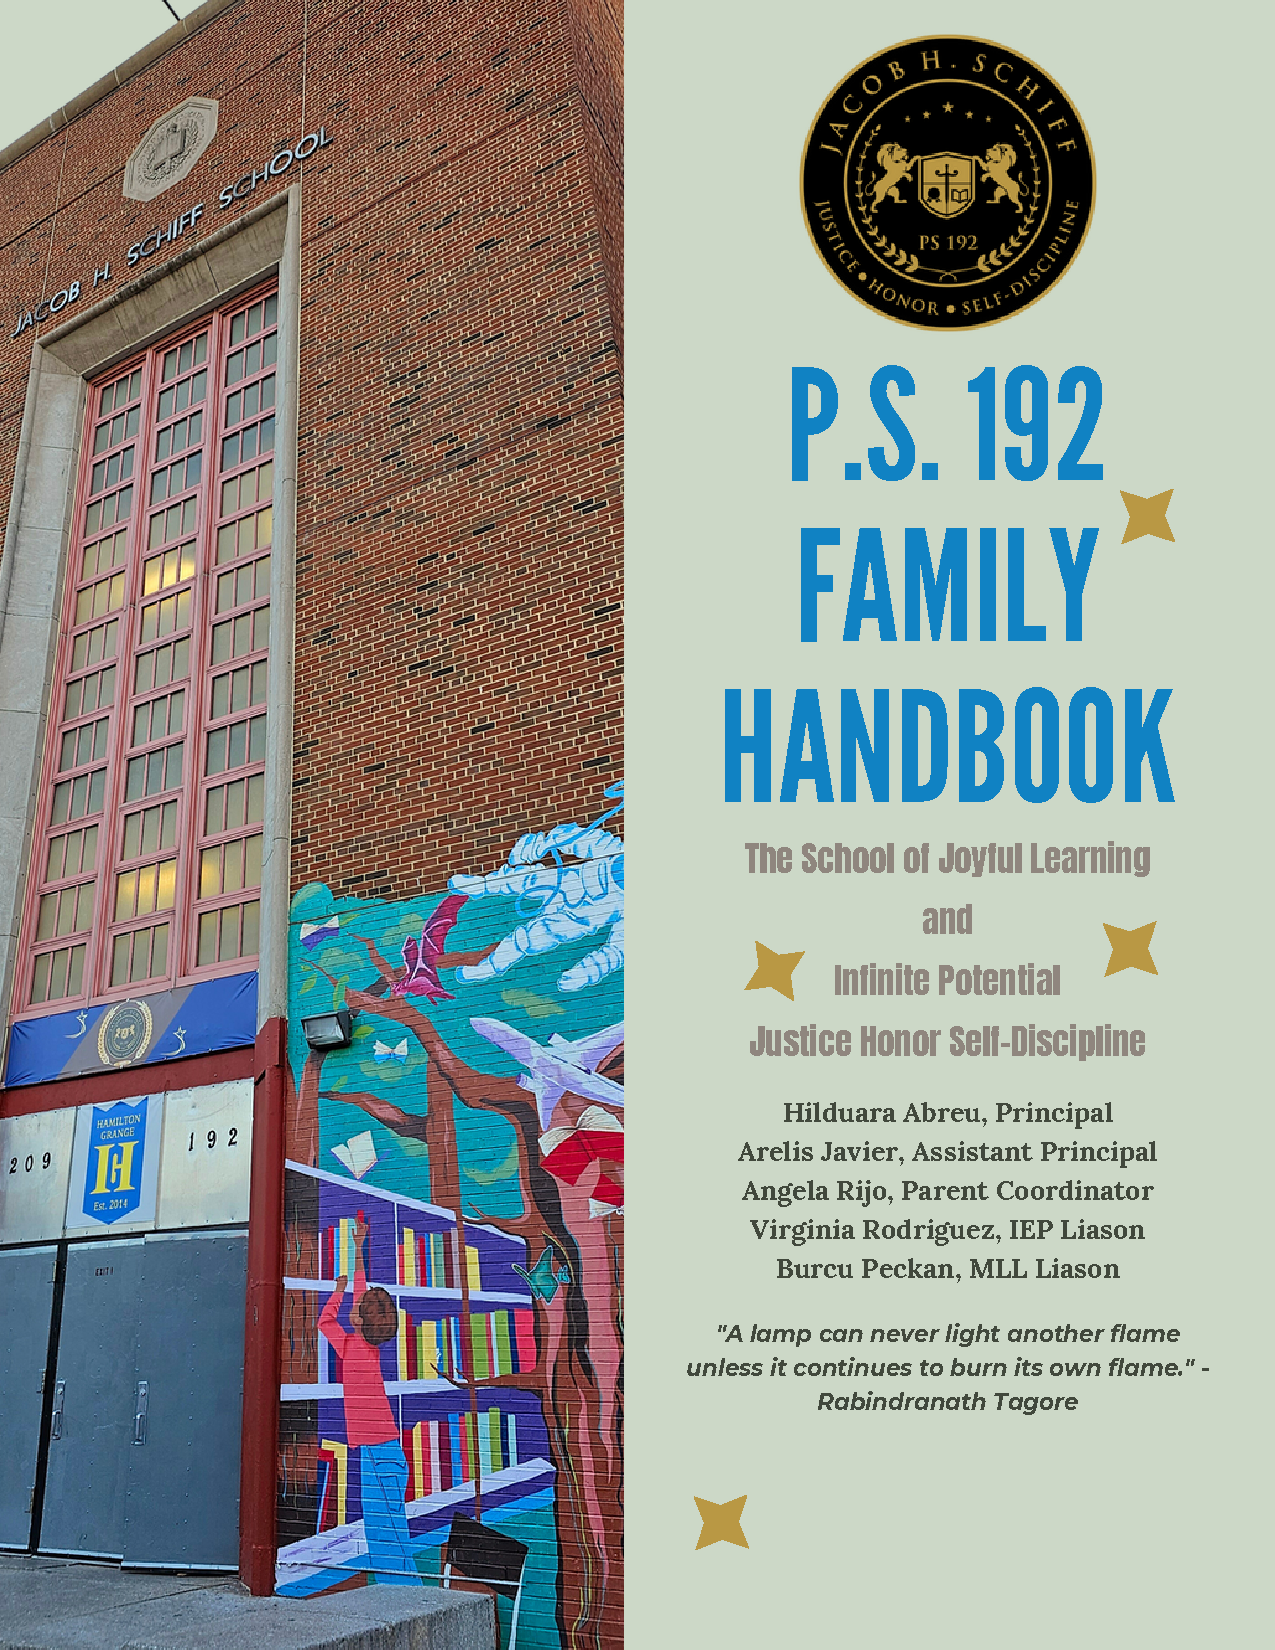
\includepdf[pages=1,fitpaper]{pdf.pdf}

\pagenumbering{\fancyhf{}}
\pagestyle{headings}
\pagenumbering{arabic}

\fancyhead[R]{\thepage}

\fancyfoot[C]{The School of joyful Learning \& Infinite Potential}
\pagestyle{fancy}
\renewcommand{\footrulewidth}{1px}

\definecolor{dkgreen}{rgb}{0,0.6,0}
\definecolor{gray}{rgb}{0.5,0.5,0.5}
\definecolor{mauve}{rgb}{0.58,0,0.82}

\clearpage
\clearpage \tableofcontents \clearpage

\section{1 Message From Principal Abreu}
\label{sec:orgb8a5b73}

Dear Staff:

Welcome to the 2023-2024 edition of the PS 192: Jacob H. Schiff Faculty and Staff Handbook. It is the responsibility of each staff member to be fully acquainted with the information contained herein. This handbook is a living document and it will be updated, as necessary, throughout the year. It is meant to provide information and procedures that are important for the smooth operation of our PS 192 community. This handbook is a guide for ALL STAFF MEMBERS about the daily operation of our school. Please familiarize yourselves with your individual and school-wide responsibilities. Please do not hesitate to ask questions or get further clarification regarding any policy or procedure.

I encourage you to begin by thoroughly acquainting or re-acquainting yourself with our school’s philosophy, mission, objectives, and core principles, as outlined in the School Overview. Key elements of this vision are elaborated upon throughout the handbook, along with important information about structures and policies that support our school mission and ensure the safety and success of all members of our school community.

During the upcoming school year, we will continue to strengthen and deepen our work in relation to NYCDOE and District 6 priorities, as reflected in our School Problem of Practice, priorities, and CEP Goals. These areas will be central to our work as a Professional Learning Community and will be further addressed in Professional Learning sessions and Professional Planning Teams, as well as in administrative memos and guidelines, many of which can be accessed in Appendix B of this handbook.

I look forward to our continued collaboration in the year ahead.

With Justice, Honor and Self-Discipline,


\includegraphics[width=100px]{/home/rob/ps192_welcome_letters/ps192_family_handbook/hil_signature.png}

\textbf{\textbf{Hilduara Abreu, Principal}}

\textbf{\textbf{The School of Joyful Learning!}}

\href{https://www.ps192.org}{www.ps192.org}

\begin{figure}[b]
\begin{center}

\includegraphics[width=40mm,scale=0.3]{ps192.png}
\caption{PS 192 school logo}
\label{fig:school_logo}
\end{center}
\end{figure}

\clearpage

\section{2 Acknowledgment of Receipt and Review}
\label{sec:orge7f493e}

\textbf{Date: September, 2024}

\textbf{Subject: Faculty and Staff Handbook Acknowledgment of Receipt and Review}
\vspace*{1cm}

I,:\line(1,0){150}(staff member name), hereby acknowledge that I have read and understand the contents of the  Faculty and Staff Handbook, including Appendix A: Chancellor’s Regulations, as well as the PS 192  Family Handbook and Citywide Behavioral Expectations to Support Student Learning.  I understand that I am also responsible for following the directives included in Appendix B: Administrative Memos, as well as subsequent administrative directives that may be issued during the year. I will adhere to the policies and procedures set forth in the PS 192 Faculty and Staff  Handbooks, the Chancellor’s Regulations and in all Administrative Memos.

\vspace{3mm}

\faSquareO \hspace{1em} I have reviewed The P.S. 192 Staff Handbook

\vspace{10mm}

\begin{center}
\noindent\begin{tabular}{ll}
\makebox[2.5in]{\hrulefill} & \makebox[2.5in]{\hrulefill}\\
Teacher's Signature & Date\\[8ex]% adds space between the two sets of signatures
\makebox[2.5in]{\hrulefill} & \makebox[2.5in]{\hrulefill}\\
Assistant Principal & Date\\[8ex]% adds space between the two sets of signatures
\end{tabular}
\end{center}
\begin{figure}[b]
\begin{center}

\includegraphics[width=80mm,scale=0.8]{static/himher1}
  \label{fig:school logo}
\end{center}
\end{figure}
\clearpage

\section{3 School Overview}
\label{sec:orged71db3}

\subsection{3.1 Core Values}
\label{sec:org3672db3}

At P.S. 192, we uphold a set of core values that serve as the foundation of our educational community. These values, rooted in the principles of justice, honor, and self-discipline, guide our actions, decisions, and interactions, creating a culture of integrity and excellence.

\begin{wrapfigure}{l}{0.43\textwidth}
    
\includegraphics[width=0.45\textwidth]{static/logohim.png}
    \caption{The lion's den}
    \label{fig:yourlabel}
\end{wrapfigure}
\begin{itemize}
\item \textbf{\textbf{Justice:}} We are committed to fairness and equality for all members of our school community. We believe in the equitable treatment of every individual, irrespective of their background, ensuring that each student has the opportunity to thrive academically and personally. Our commitment to justice fosters an inclusive and supportive environment where every voice is heard, valued, and respected.

\item \textbf{\textbf{Honor:}} Integrity is the cornerstone of our educational philosophy. We encourage our students to act with honesty and integrity in all aspects of their lives. Upholding honor means taking responsibility for one’s actions, demonstrating ethical behavior, and consistently adhering to a code of moral values. We believe that integrity is the pathway to personal growth and societal betterment.

\item \textbf{\textbf{Self-Discipline:}} We recognize the importance of self-control and self-mastery in achieving success. At P.S. 192, we instill in our students the value of self-discipline as an essential skill for achieving their goals and aspirations. Through self-discipline, our students learn to set priorities, manage their time effectively, and overcome challenges, ultimately becoming responsible and accountable individuals.
\end{itemize}

These core values of justice, honor, and self-discipline guide us in pursuing academic excellence and character development. By embracing these principles, we empower our students to become responsible citizens, compassionate leaders, and lifelong learners who contribute positively to our global community.

\subsection{3.2 Vision}
\label{sec:org167b811}

To ensure all students acquire the essential knowledge and skills they need to become independent thinkers, active participants, and contributors in their roles as students and as members of society.

\subsection{3.3 Mission}
\label{sec:orgbf0476c}

To provide a welcoming, safe, resourceful, and nurturing environment that supports our school community’s academic and social-emotional development where children are respected and engaged in challenging curricula that motivate them to realize their potential as active, lifelong learners. Through our guiding core values of Justice, Honor, and Self-discipline, we aspire to promote perseverance, love, empathy, and respect for oneself and others.

"Good, better, best. Never let it rest until your good is better, and your better is best." -St. Jerome
\section{4 Educational Philosophy}
\label{sec:org285b5cd}

We believe that relationships, with oneself and with others, form the basis of learning and teaching. These relationships extend beyond the classroom to include children’s families and the multiple communities of which they are a part. By building meaningful relationships among school, home, and the wider community, we seek to instill in each child an integral sense of continuity and connection that will support his or her growth in its many dimensions.

Learning is a natural human process inherent to all children, transcending cultural, socio-economic, and learning differences. Children’s innate interests and capabilities are essential to the learning process. A stimulating and engaging environment can awaken a sense of wonder and intellectual curiosity that must be carefully guided and fed. Students learn best when teachers draw upon their existing understandings and help them build new understandings based on increasingly complex knowledge. To this end, our school integrates child-centered pedagogies with rigorous, content-rich instruction in response to ongoing assessment of individual student needs.

\subsection{4.1 Core Principles}
\label{sec:org6365faf}

The vision for Jacob H. Schiff is guided by the following core principles:

\begin{itemize}
\item An effective learning environment places meaningful relationships—among teachers, students, families, and other community members—at its center.

\item Small learning communities, in which adults and children know each other well, provide rich opportunities for personal, social, and intellectual development.

\item Families play an essential role in their children’s education and should therefore be invited to participate in multiple aspects of school life.

\item A community-based school must be accessible, accountable, and responsive to all families, regardless of their linguistic, cultural, socio-economic, or educational backgrounds.

\item Children benefit from a coherent academic program that encompasses Pre-Kindergarten to Grade 5.

\item All children have gifts and talents, which can be effectively fostered in heterogeneous classrooms in which adults hold high expectations for every student.

\item Children learn through active engagement and exploration, and by constructing understandings based on their own experiences and observations.

\item A language-rich environment, accessible to children of diverse backgrounds, provides the foundation for achievement in all academic disciplines and areas of life.

\item A well-rounded education provides academic rigor as well as opportunities for self-expression, artistic creation, and personal reflection.

\item Engagement in multicultural, multilingual learning environments will prepare children to participate fully in our diverse society. Education should include not only the mastery of information and skills, but also the development of critical thinking abilities and ethical awareness.
\end{itemize}

\subsection{4.2 Commitment to Achievement}
\label{sec:orga90ae79}

In our commitment to delivering a rigorous, inclusive, and family-centered educational experience for the children of our community, PS 192 will:

\begin{itemize}
\item Uphold our identity as a dedicated learning community, earnestly striving to intimately understand each student and their family.

\item Cultivate an intellectually stimulating and captivating learning environment that prioritizes relationships as the primary conduit of both learning and teaching.

\item Assure that our students consistently attain and surpass academic benchmarks across all subject areas.

\item Incorporate family involvement and feedback at various levels of school administration.

\item Instill in every student elevated expectations for their own capabilities, reinforced by unwavering belief in their demonstrated aptitudes.

\item Conduct methodical evaluations of student learning assessments with the aim of scrutinizing data for patterns of misunderstandings and devising solutions to enhance student achievement.
\end{itemize}

\subsection{4.3 Commitment to Parental Engagement}
\label{sec:org7892d2e}

Research consistently confirms that meaningful family engagement plays a pivotal role in the academic success of children. In light of this, Jacob H. Schiff holds family engagement and authentic home-school partnerships at the core of its mission.

At Jacob H. Schiff, we actively promote meaningful family engagement through regular opportunities for family involvement in classroom activities and school events. Our program design ensures that such involvement aligns with both the school’s mission and the educational objectives set by our teachers and staff. Parents and other family members are encouraged to provide various forms of support, which may include preparing classroom materials, delivering curriculum-related presentations about their family experiences or cultural backgrounds, or sharing their expertise in areas such as music, dance, storytelling, science, or technology. Through these collaborative efforts, teachers and family members can establish mutual respect as valued partners in the education of all PS 192 students.

The relationship between the school and families is central to our mission. Consequently, we aspire to foster an active partnership that leverages the unique resources each student brings from their home environment. When families are deeply engaged in their children’s learning and children witness their parents’ dedication to their education, a vital connection is forged between the home and the school. By cultivating a cooperative partnership with each student’s family, our goal is to emphasize the role of families as the ultimate stakeholders in the school and acknowledge their responsibility in the comprehensive education of each child.

As part of our commitment to transparent communication, each grade group is expected to send newsletters to families via grade-level Google groups at least twice a month. These newsletters will provide updates on curriculum developments within the classroom, upcoming field trips, suggestions for family outings, and recommended books to enhance your understanding of your child’s educational journey within our school.

We look forward to nurturing this strong partnership with you and working collaboratively to ensure the success and well-rounded development of all our students.

\subsection{4.4 Commitment to Community Engagement}
\label{sec:org7a37eba}

Distinguished educational institutions not only serve as sources of inspiration for students but also maintain intrinsic connections with the communities in which they are situated. A comprehensive and diverse educational program is enriched through hands-on learning, both within and beyond the confines of the classroom. Through the establishment of cooperative alliances with community organizations, our objective is to enhance the Academy’s academic curriculum with genuine learning opportunities, extracurricular activities, and avenues for community engagement. Consequently, students can establish profound links between the school and the broader community, fostering their personal, social, and ethical growth, in addition to supporting their academic achievements. This communication aims to inform parents of our commitment to this holistic approach to education.

\subsection{4.5 Promoting Positive Student Behavior}
\label{sec:org6752b16}

School culture and climate have a profound impact on students’ academic progress and their relationships with peers and adults. Each teacher is expected to promote a positive school culture that provides students with a supportive environment in which to grow both socially and academically. Teachers are expected to take a proactive role in nurturing students’ pro-social behavior. Social emotional learning must is one of the components of a school’s program of universal prevention for all students.

Effective social emotional learning helps students develop fundamental life skills, including:

\begin{itemize}
\item Recognizing and managing emotions

\item Developing caring and concern for others

\item Establishing positive relationships

\item Making responsible decisions

\item Handling challenging situations constructively and ethically
\end{itemize}

When students develop these skills, they experience more positive relationships with peers, engage in more productive social behaviors, and are less likely to engage in misconduct.

\subsection{4.6 Social, Emotional, and Ethical Education}
\label{sec:org2a082a7}

Research findings support Jacob H. Schiff’s emphasis on fostering social, emotional, and CASEL ethical competencies as substantial contributors to academic achievement. When these educational processes are integrated with academic instruction, students gain the essential tools necessary for a lifelong commitment to learning and responsible citizenship. Therefore, it is imperative that WHA teachers actively incorporate these skills throughout all facets of the curriculum. Collaboration between teachers, school staff, and family members is essential to collectively develop and exemplify the adult competencies we aspire for our children to emulate.

\subsection{4.7 The Pre-Kindergarten–Grade 5 Looping Model}
\label{sec:org86c1081}

Jacob H. Schiff has been implementing since 2021, offers students a continuous elementary learning experience—a model that holds value for many families and aligns with educational research. Looping, as defined by Cistone et al. (2004) in Hill (2018, p. 2), is "a policy in which whole classes (or most of the students within a class) are taught by the same teacher in sequential years." This practice, also known as "continuous learning," has demonstrated both quantitative and qualitative benefits within a school setting. A recent seminal study shows that looping can lead to improved test scores, with the most significant effects observed among minority students (Hill 2018, p. 2, Franz et al. 2010, Cistone et al. 2004, Bogart, V. 2002). Furthermore, it positively impacts student attendance and their progression to the next grade (Cistone, et al. 2004).

Daggett’s Effectiveness and Efficiency Framework highlights classroom looping as one of the practices worth considering, ranking it second on the list (Beilefeld 2016). Daggett presents looping as a "low-cost, high-effect" approach for modern schools, a sentiment echoed by Hitz (2007), who emphasizes that looping is not a complex undertaking. Looping contributes to a positive school culture by reducing transitions and increasing trust in relationships with students and parents (Rassmussen 1998, Chaika 2009).

Schools that have effectively implemented the looping structure have reported several benefits, including improved relationships among students and between teachers and students, more efficient instruction, improved attendance rates (5\%), reduced student grade level retention (43\%), fewer referrals of students to special education programs (55\%), and improved student discipline (Grant 2017). Staff attendance also improved, with an average reduction from 7 days absent to just 3 days absent (Grant 2017).
\section{5 School Day Procedures}
\label{sec:orgaaa2446}

\subsection{5.1 Lesson Plans}
\label{sec:org159c693}

Effective lesson planning is the cornerstone of a successful instructional day. It allows us to set clear goals, organize instructional strategies, and discussion protocols, and ensure that we are delivering quality education to our students. By planning your lessons in advance, you not only optimize instructional time but also create a more engaging, data-driven, and focused learning environment for our students.

Every staff member has been granted access to a printer, printing paper, ink, and a lesson plan binder to facilitate an effortless process of keeping your lesson plans accessible and organized when requested by an administrator. Printing the daily plans in advance further contributes to a smoother operation within the classrooms. It minimizes disruptions during instructional time.

I understand that we all have busy schedules, and sometimes it can be challenging to find the time for detailed lesson planning. However, I want to remind you that our commitment to our students’ success is what drives us. Taking the time to use your student data to plan whole group and target small group instruction is not just our contractual and professional duty but also our moral responsibility.

Your daily Lesson plan must include the following elements:

\begin{itemize}
\item \textbf{\textbf{Objective(s):}} Clearly define the learning objectives, target, or goals of the lesson. What should students know or be able to do by the end of the lesson? “I can\ldots{}”

\item \textbf{\textbf{Standards:}} Reference the relevant academic standards that align with the lesson.

\item \textbf{\textbf{Duration:}} Indicate the estimated time needed to complete each section of the lesson.

\item \textbf{\textbf{Materials and Resources:}} List all materials, resources, and technology required for the lesson, including textbooks, workbooks, multimedia, or any other tools.

\item \textbf{\textbf{Pre-assessment:}} Describe how you will assess students’ prior knowledge or skills related to the lesson topic.

\item \textbf{\textbf{Integration:}} If relevant, indicate how the lesson integrates with other subjects or disciplines.

\item \textbf{\textbf{Safety Considerations:}} Include any safety precautions or considerations if they apply to the lesson.

\item \textbf{\textbf{Introduction:}} Explain how you will engage students and introduce the lesson’s main concept or topic.

\item \textbf{\textbf{Instructional Strategies:}} Outline the teaching methods, strategies, and activities you will use to convey the lesson content. Be sure to include differentiated approaches to meet the needs of diverse learners.

\item \textbf{\textbf{Grouping and Differentiation:}} Specify how students will be grouped, whether by ability, interest, or other criteria. Describe how you will differentiate instruction to meet the needs of various learners, including those who may need additional support or challenges.

\begin{itemize}
\item \textbf{\textbf{Accommodations and Modifications:}} Detail any accommodations or modifications for students with special needs or diverse learning styles.

\item \textbf{\textbf{Language Support:}} Describe how you will support English language learners (ELLs) or students who require language assistance.

\item \textbf{\textbf{Engagement and Discussion Strategies:}} Highlight strategies and discussion protocols to keep students cognitively engaged and motivated throughout the lesson.
\end{itemize}

\item \textbf{\textbf{Assessment and Formative Assessment:}} Specifically name and describe the methods you will use to assess students’ understanding during the lesson. Include both formative assessments (ongoing checks for understanding) and a summative assessment to evaluate the lesson’s overall success.

\item \textbf{\textbf{Closure:}} Explain how you will wrap up the lesson, summarize key points, and connect the content to the learning objectives.

\item \textbf{\textbf{Homework or Follow-Up:}} Specify any homework assignments or follow-up activities that students should complete outside of class.

\item \textbf{\textbf{Cluster Teachers:}} Specify the class for which the lesson is designed. For example, Class 201. Each lesson plan must be tailored to the needs of each individual class.

\item \textbf{\textbf{Optional Best Practice Tip:}} Reflection: Provide space for reflection on the effectiveness of the lesson and any adjustments you might make when teaching it again.
\end{itemize}

Let’s remember our shared dedication to providing an excellent education for PS 192 students. By prioritizing lesson planning and printing daily plans, we are not only making our jobs easier but also contributing to the overall social, emotional, and academic growth and success of our students.

If you have any questions or need any of the resources listed in this email, please don’t hesitate to reach out to Ms. Macdonald, Ms. Rodriguez, or me. We are here to support you and work as a team to achieve our goals.

Together, we can create an exceptional learning experience for all of our students.

\subsection{5.2 Arrival}
\label{sec:org172739b}

Breakfast is served within the cafeteria from 7:40 to 7:55 am. If a student intends to partake in breakfast at school, they should enter the cafeteria during the designated time frame of 7:40 to 7:55 am. School staff will ensure that students who choose to have breakfast at school are escorted to their respective classrooms by 7:59 am.

All students in grades K-5 are required to assemble in the yard during arrival. Parents are kindly requested not to accompany their child into the school building. However, on the first day of school, Kindergarten and transfer students may be accompanied by a parent/guardian into the school.

Please be mindful of our shared facility with PS 209 during both Arrival and Dismissal. To maintain a smooth flow, we should refrain from entering the school front door during the arrival or dismissal times of PS 229, which occur 10 to 20 minutes before our own. PS 192 families are kindly asked to wait until a PS 192 staff member opens the gate before entering.

\subsection{5.3 Student Attendance}
\label{sec:orgdddd1b4}

Children cannot attain their full potential, both academically and socially, if their attendance exhibits irregularity. The absence of consistent participation in instruction and the disruption of their ability to form connections with peers and curriculum significantly jeopardizes a child’s developmental progress.

Students arriving late find themselves endeavoring to catch up with the classroom’s tone and pace. Therefore, we strongly urge parents to accord utmost importance to both attendance and punctuality.

Our school policy stipulates that students should be present in school every day from 8:00 AM to 2:20 PM. There is a brief grace period of 5 minutes, and no student should be marked as late until after 8:05 AM. In cases of late arrivals, Shalymet Cuesta maintains records in our attendance notebook, which serves as a supplementary record. If a child has been initially marked as absent, kindly ensure that the attendance sheet is amended to reflect lateness. If the attendance folder has already been submitted, any recorded absence will be duly adjusted to reflect lateness by Shalymet Cuesta in the main office.

Each class is equipped with an attendance folder that contains the scan sheet and a comprehensive list of students. Teachers bear the responsibility of meticulously recording student attendance. In the event of concerns regarding a student’s attendance, teachers should initially engage in direct communication with the parent(s)/guardian(s). Should the issue persist, teachers are encouraged to escalate it to Rijo, Cuesta, or Estrella. If the problem remains unresolved, please contact Javier.

Please take note that excessive absences and/or tardiness may be construed as educational neglect, warranting reporting to the New York State Agency for Child Services (ACS).

Upon completion of attendance, it is imperative to dispatch the attendance folder to the school office by 9:15 AM.

\begin{itemize}
\item The folder will be made available in each teacher’s mailbox prior to 8:00 AM. In the event that it is not found in your mailbox by 8:00 AM, it will be delivered directly to your classroom.

\item Attendance must be recorded promptly upon the class’s entry into the room, and attendance forms must be diligently completed on a daily basis, serving as a vital backup for our records.

\item To ensure that attendance data is entered into the Attendance Tracking System (ATS) before the daily deadline, the attendance folder must be returned to the school office no later than 9:15 AM, with the classroom teacher(s) ultimately responsible for verifying its accuracy.
\end{itemize}

It is of paramount importance that attendance is meticulously documented, as these records constitute official and legal documents of the highest significance.
\section{6 Crisis Intervention Plan}
\label{sec:org59c1722}

\subsection{6.1 What is Tier 1 Support?}
\label{sec:org5245db1}

Tier 1 systems, data, and practices support everyone across all settings. They establish the foundation for delivering regular, proactive support and preventing unwanted behaviors. Tier 1 emphasizes modeling, teaching, and acknowledging positive social, emotional, and behavioral (SEB) skills.

The core principles guiding Tier 1 include the understanding that we can and should:

\begin{itemize}
\item Effectively teach appropriate SEB skills to all students.

\item Differentiate instruction for behavior.

\item Intervene early before unwanted behaviors escalate.

\item Use research-based, scientifically validated interventions whenever possible.

\item Clearly define consequences for unwanted behaviors.

\item Monitor student progress.

\item Use data to make decisions.
\end{itemize}

\subsection{6.1.1 Tier I De-Escalation Strategies}
\label{sec:orgdbdf026}

\begin{itemize}
\item Act calm.

\item Give a choice—a simple, quick, calm, respectful way of letting a student know about the unwanted behavior and what they could do instead.

\item Change the subject to a positive one: Redirect behavior.

\item Remind them of a strategy they know.

\item Co-regulate when they can self-regulate.

\item Invite students to a calming activity (breathing, drawing, journaling).

\item Give space and wait time.

\item Use a behavior progress report (must be signed by a parent on a daily or weekly basis).

\item 1-1 conference with the student and/or guardian.
\end{itemize}

\subsection{6.2 What is Tier 2 Support?}
\label{sec:org1f6a778}

\begin{itemize}
\item Progress monitoring for at-risk students.

\item Create structures and predictability: Intervene early before unwanted behaviors escalate by anticipating triggers and possible solutions.

\item Weekly meeting with the Crisis Intervention team for increasing contingent adult feedback.

\item Analyze academic and behavioral performance.

\item Increase home/school communication.

\item Collect and use data for decision-making.

\item Basic-level function-based support.
\end{itemize}

\subsection{6.2.1 Tier II De-Escalation Strategies}
\label{sec:org8939cc0}

\begin{itemize}
\item Act calm.

\item Be empathetic and nonjudgmental.

\item Avoid overreacting.

\item Set positive limits.

\item Ignore challenging questions.

\item Allow quiet time for reflection.

\item Do a quick body scan.

\item Use diffusers to de-escalate.

\item Practice reflective teaching.

\item 1-1 conference with students and/or guardian.

\item Small group counseling sessions.
\end{itemize}

\subsection{6.3 Tier 3}
\label{sec:orga194511}

Tier 3 involves intensive, individualized interventions for students with significant behavioral needs that have not responded to Tier 1 or Tier 2 supports.

\section{7 Professional Expectations}
\label{sec:orgdf1756a}

\subsection{7.1 Teacher Criteria}
\label{sec:org5922fb3}

At Jacob H. Schiff, a foundational tenet of our educational philosophy revolves around a team-based approach to teaching and learning. In alignment with our school’s overarching mission, our dedicated educators engage in collaborative efforts to meticulously design curriculum and instructional strategies. They employ a diverse array of assessment tools to thoughtfully analyze student progress, thereby informing and enhancing our teaching methods.

This collaborative planning plays a pivotal role in ensuring the seamless alignment of curriculum objectives and fostering instructional uniformity across various classrooms and grade levels. Furthermore, our teachers operate within collaborative teams to actively support the holistic growth of our students, encompassing their social, emotional, and ethical development. This comprehensive approach underscores our commitment to providing a well-rounded education for your child.

All personnel are expected to embrace and promote the mission, philosophy, and fundamental tenets of PS 192: Jacob H. Schiff, and must either possess or be open to acquiring the following skills and attitudes:

\begin{itemize}
\item Operate effectively within a highly collaborative environment, necessitating active, suitable, and proficient communication with peers, parents, students, and other stakeholders.

\item Adapt to the school’s timetable and organizational structure, tailored to meet the diverse backgrounds and requirements of our students.

\item Engage in interdisciplinary planning and teaching teams with a primary focus on integrating social and emotional learning into every facet of instruction.

\item Adopt an open-door policy to foster the development of best-practice pedagogy and facilitate professional growth through collaboration.

\item Utilize a variety of assessment methods and student data to guide effective instruction.

\item Review, apply, and ensure the provision of services, modifications, and accommodations as outlined in IEPs (Individualized Education Plans) for SWD (Students with Disabilities) in compliance with their entitlements.

\item Effectively manage classrooms populated with diverse learners, utilizing flexible and cooperative groupings, as well as targeted whole-class instruction to address varying learning styles, academic proficiency levels, and social-emotional needs.

\item Incorporate project-based work and instruction across various content areas.

\item Devise and execute challenging, engaging units that encourage critical thinking and culminate in completed student works, contributing to a growing portfolio.

\item Seamlessly integrate technology as a teaching tool within the classroom.

\item Create meaningful opportunities for family involvement within the classroom and throughout the school, including workshops and resources.

\item Contribute to and participate in special programs, such as workshops and curriculum nights, with a particular emphasis on engaging families.

\item Engage in after-school and Saturday programs, attend planning sessions, and potentially contribute to summer planning and curriculum development.

\item Report to the assigned post by 8:00 a.m. daily, as any arrival after 8:00 a.m. will be considered tardy.

\item Adhere to the prescribed program schedule, punctuality in all classes, Related Services sessions, and fulfill all assigned duties and responsibilities.

\item Maintain readily accessible daily lesson plans or session plans upon request, utilizing a provided lesson plan binder for organization and accessibility, which should be placed atop the portfolio shelf near the entrance.

\item Regularly check and respond to emails and review the office communication board.

\item Attend to office mailboxes at the start and end of each day. When departing the building for lunch or meetings, ensure completion of the sign-out book and consult with our secretary, Ms. Dulce Infante, before leaving.

\item Following attendance at professional learning sessions or workshops during work hours, provide proof of attendance and an agenda within 48 hours to Ms. D. Infante, in either hard or soft copy format. Initiate daily attendance taking at the outset of each day, preserving records and placing the red attendance folder in the exterior compartment adjacent to your classroom door. This requirement applies solely to classroom teachers and substitute teachers.

\item Complete the sign-out book, situated at the classroom entrance, when removing a student from the classroom for the provision of Related Services or evaluation.

\item Maintain close supervision of students at all times. During the school day, students are not permitted to exit the school premises unless signed out at the welcome center by an adult aged 18 or older, whose name must be listed on the emergency contact card. Outside of dismissal hours, teachers may not release a child to anyone not listed on the blue card without administrative approval. The official teacher is responsible for the whereabouts of their assigned students at all times. Should another staff member redirect a student, the homeroom teacher must be informed. Students from different classes should not enter your classroom without prior notification via classroom phone or written communication. In grades 4-5, students may travel within the building independently with a pass, but they must never be left unattended. In the event of leaving the room, students must be entrusted to the care of another adult. In emergencies, contact the main office, a supervisor, or another staff member for assistance. Group movement of students within the building must always include adult accompaniment. Under no circumstances should students be left unattended in hallways or anywhere within the building. Immediate notification to the main office is imperative in the following situations:

\begin{itemize}
\item if a student departs from your room without permission.

\item fails to return from lunch or a bathroom break.

\item or goes missing for a duration exceeding 5 minutes, in order to promptly inform their parents and seek their assistance in locating the student.
\end{itemize}

\item When encountering a student without an adult or pass, direct them back to their assigned classroom or escort them to the main office if no classroom is evident. No students should be permitted to walk the hallways or leave the building without a classroom pass.
\end{itemize}

\section{8 Professional Conduct}
\label{sec:org4e6bd3d}

\subsection{8.1 Unacceptable Professional Behaviors}
\label{sec:orgb996c2c}

\begin{itemize}
\item Displaying confrontational, dismissive, or disrespectful behavior toward students, colleagues, or parents.

\item Engaging in any conduct that undermines the dignity, respect, or safety of the school environment.

\item Neglecting duties or failing to perform responsibilities as outlined in the job description or the school’s policies and procedures.

\item Failing to comply with attendance policies, including arriving late or leaving early without proper authorization.

\item Inappropriate use of technology or resources provided by the school for personal purposes during work hours.

\item Failing to maintain professional boundaries with students and colleagues.

\item Engaging in behavior that could be construed as favoritism, discrimination, or harassment.

\item Failing to adhere to the confidentiality policies regarding students, staff, or school operations.

\item Any other conduct deemed unprofessional or detrimental to the school community.
\end{itemize}

\section{9 Health and Wellness}
\label{sec:org81107e6}

\subsection{9.1 School Nurse}
\label{sec:org4166b4e}

The school nurse is responsible for managing student health issues, administering medication, and providing first aid. Teachers should send students to the nurse with a pass, unless it is an emergency.

\subsection{9.2 Administration of Medication}
\label{sec:orgce5c2fc}

Students who require medication during school hours must have a completed 504 plan on file. The nurse is the only individual authorized to administer medication to students.

\subsection{9.3 Illness}
\label{sec:org3bd1d6e}

If a student is feeling unwell, they should be sent to the nurse for evaluation. If the student is too ill to remain in school, the nurse will contact the parents/guardians to arrange for the student to be picked up.

\subsection{9.4 Incident Reports}
\label{sec:org5185d32}

In the event of an accident or injury, staff members must complete an incident report and submit it to the school nurse and administration. This report should include details of the incident, the individuals involved, and any actions taken.

\subsection{9.5 Safety and Emergency Preparedness}
\label{sec:org95fd3f6}

Safety is a top priority at PS 192. All staff members must be familiar with the school’s emergency procedures and participate in regular drills. In case of an emergency, follow the established protocols to ensure the safety of students and staff.

\subsection{9.6 Inter-visitations}
\label{sec:orgb6e98dc}

Inter-visitations between teachers are encouraged to promote professional growth and the sharing of best practices. Teachers interested in participating in inter-visitations should coordinate with their grade-level team and administration.

\subsection{9.7 Safety}
\label{sec:org9350d84}

The safety of our students and staff is of the utmost importance. All staff members must adhere to safety protocols, including supervising students at all times, ensuring that students are not left unattended, and reporting any safety concerns to the administration immediately.

This completes the conversion of the entire document into Org mode. If you need any further modifications or have any additional requests, please let me know!
\end{document}
